\documentclass{beamer}

\usepackage[french]{babel}
\usepackage{csquotes}
\usepackage{xcolor}
\usepackage{mdframed}
\usepackage{fontawesome}
\usepackage[T1]{fontenc}
\usepackage{pgf,tikz}


\usetikzlibrary{shapes}
\usetikzlibrary{arrows}
\tikzset{
  font={\fontsize{7pt}{12}\selectfont}}
\usetikzlibrary{graphs}


\graphicspath{{./images/}}

\definecolor{lightgray}{RGB}{150,150,150}
\definecolor{shadecolor}{RGB}{255,241,204}

\mdfdefinestyle{yellowbox}{%
    linecolor=white, linewidth=0pt,
    backgroundcolor=shadecolor,
    leftline=false, rightline=false,
    innertopmargin=0.25cm, innerbottommargin=0.25cm,
    innerleftmargin=0.25cm, innerrightmargin=0.25cm,
}

\usetheme[
        %url={nano.polymtl.ca},
        %numbering={false},
        menuwidth={0.3\paperwidth}
        ]{polymtl}

\setbeamercovered{invisible}

\begin{document}

\title[Simulation d’une voiture autonome sur le RTOS QNX]{Simulation d’une voiture autonome sur le RTOS QNX} 
%\subtitle{\vspace{1em} Présentation de l'article}
\author{ \vspace{4em} Antonin Godard et Rayan Neggazi} 
\date{\today} 
\institute{\'Ecole Polytechnique de Montr\'eal \\ 
  \vspace{-0.2em}{\small INF6600} }

\begin{frame}[plain]
  \titlepage
\end{frame}




\section{Introduction}

\begin{frame}{Table of contents}
  \tableofcontents
\end{frame}

% \begin{frame}{Résumé}
%     \begin{itemize}
%         \item Simulation d’une voiture autonome sur un système d’exploitation temps-réel QNX
%         \item Modélisation basique des parties continues et discrètes
%         \item Améliorations
%     \end{itemize}
% \end{frame}

\begin{frame}{Étapes du projet}
    \begin{enumerate}
        \item Analyse UML
        \item Modélisation TrueTime: partie discrète
        \item Simulation RTOS QNX
        \item Améliorations
        % \item Tâches \texttt{pthread}
        % \item Routine commune: \texttt{main\_worker}
    \end{enumerate}
\end{frame}

\section{Première implantation}

\begin{frame}{Cahier des charges}
    \begin{figure}
        \centering
        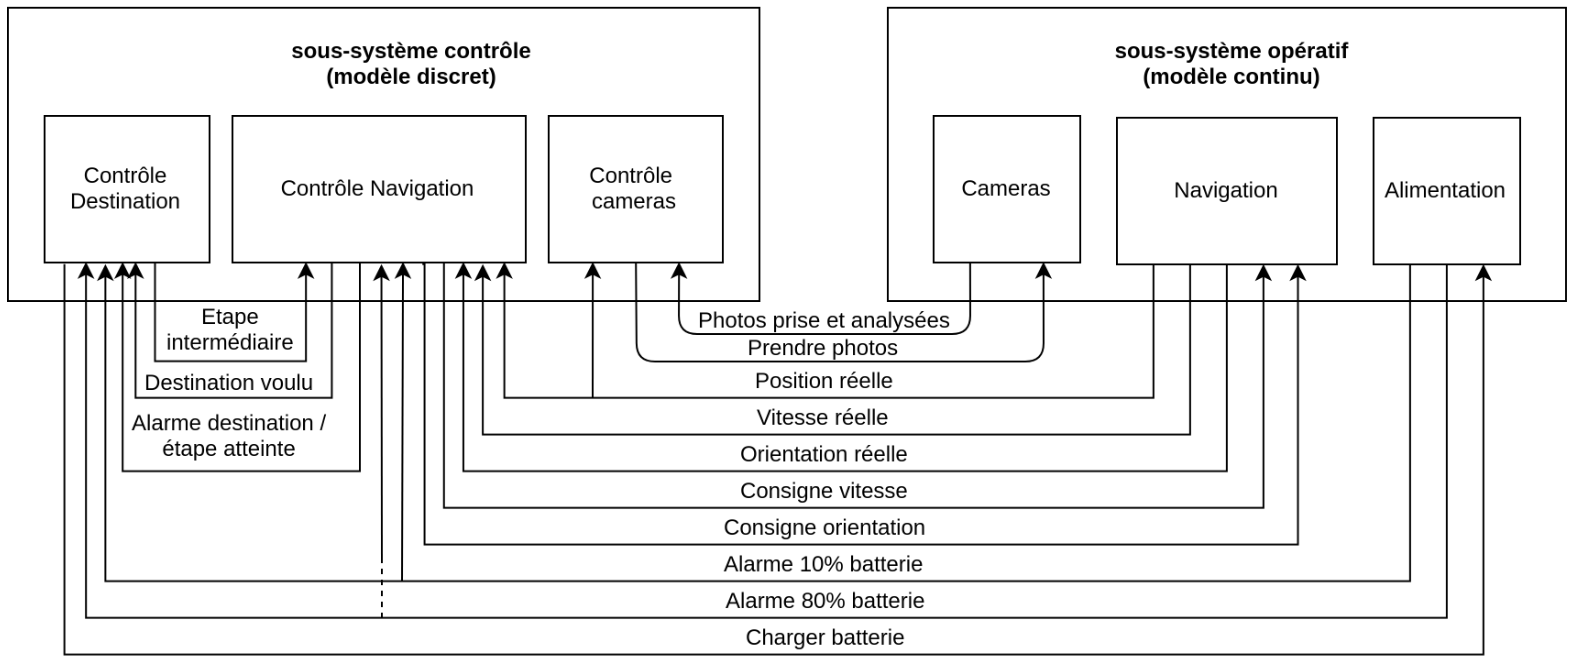
\includegraphics[width=0.9\paperwidth]{charges.png}
    \end{figure}
\end{frame}

\begin{frame}{Navigation}
    \begin{figure}[h]
        \centering
        \begin{tikzpicture}[scale = 1.3]
        
        \tikzset{edge/.style = {->,> = latex'}}
        
        % vertices
    	\node[rounded corners=3pt, draw=black, rectangle split, rectangle split parts = 2] (a)
    		at  (-2,0) {\texttt{GOTO\_DEST} \nodepart{two} {\tiny vit. = 50km/h}};
    	\node[rounded corners=3pt, draw=black, rectangle split, rectangle split parts = 2] (b)
    		at  (2,0) {\texttt{PRE\_BATTLOW}\nodepart{two} {\tiny vit. = 30km/h}};
    	\node[rounded corners=3pt, draw=black, rectangle split, rectangle split parts = 2] (c)
    		at  (2,2) {\texttt{BATTLOW}\nodepart{two} {\tiny vit. = 30km/h}};
    	\node[rounded corners=3pt, draw=black, rectangle split, rectangle split parts = 2] (d)
    		at  (-2,2) {\texttt{CHARGING}\nodepart{two} {\tiny vit. = 0km/h}};
        \node[circle, fill=black] (g) at (0,1) {};
        
        %edges
        \draw[edge] (g) to node [] {} (a);
        \draw[edge] (a) to node [above] {batt = 10} (b);
        \draw[edge] (b) to node [left] {} (c);
        \draw[edge] (c) to node [above] {closeTo(station)} (d);
        \draw[edge] (d) to node [left] {batt = 80} (a);
        
        \end{tikzpicture}
        \caption{Contrôle de la navigation}
        \label{fig:state_machine_1}
    \end{figure}
\end{frame}

\begin{frame}{Caméra et batterie}

    \begin{columns}
    
        \begin{column}{0.45\paperwidth}
            Caméra :
            \begin{itemize}
                \item Une tâche continue qui prend une photo
                \item Une tâche de contrôle pour commander la caméra (une photo tous les 10 mètres)
            \end{itemize}
        \end{column}
        
        \begin{column}{0.45\paperwidth}
            Batterie :
            \begin{itemize}
                \item Une tâche continue qui gère le niveau de batterie
                \item Deux tâches de contrôle pour les alertes
            \end{itemize}
        \end{column}
    
    \end{columns}

\end{frame}

\section{Solutions et améliorations}

\begin{frame}{Lacunes et solutions}
    
    \begin{tabular}{|c|c|}
        \hline
        \textbf{Lacune} & \textbf{Solution} \\
        \hline
        Incertitude de la périodicité des tâches
 & Ajout de timers \\
        \hline
        Variables globales pour la synchronisation & Sémaphores \\
        \hline
        Temps de simulation & Facteur d'accélération \\
        \hline
    \end{tabular}
    
    \bigskip
    
    \begin{itemize}
        \item[$\rightarrow$] Période jusqu'à 2 ms
        \item[$\rightarrow$] Synchronisation efficace
        \item[$\rightarrow$] Possibilité d'accélérer jusqu'à 100 fois 
    \end{itemize}
    
\end{frame}

\begin{frame}{Tracé avec \texttt{takePhoto}}
    \begin{figure}
        \centering
        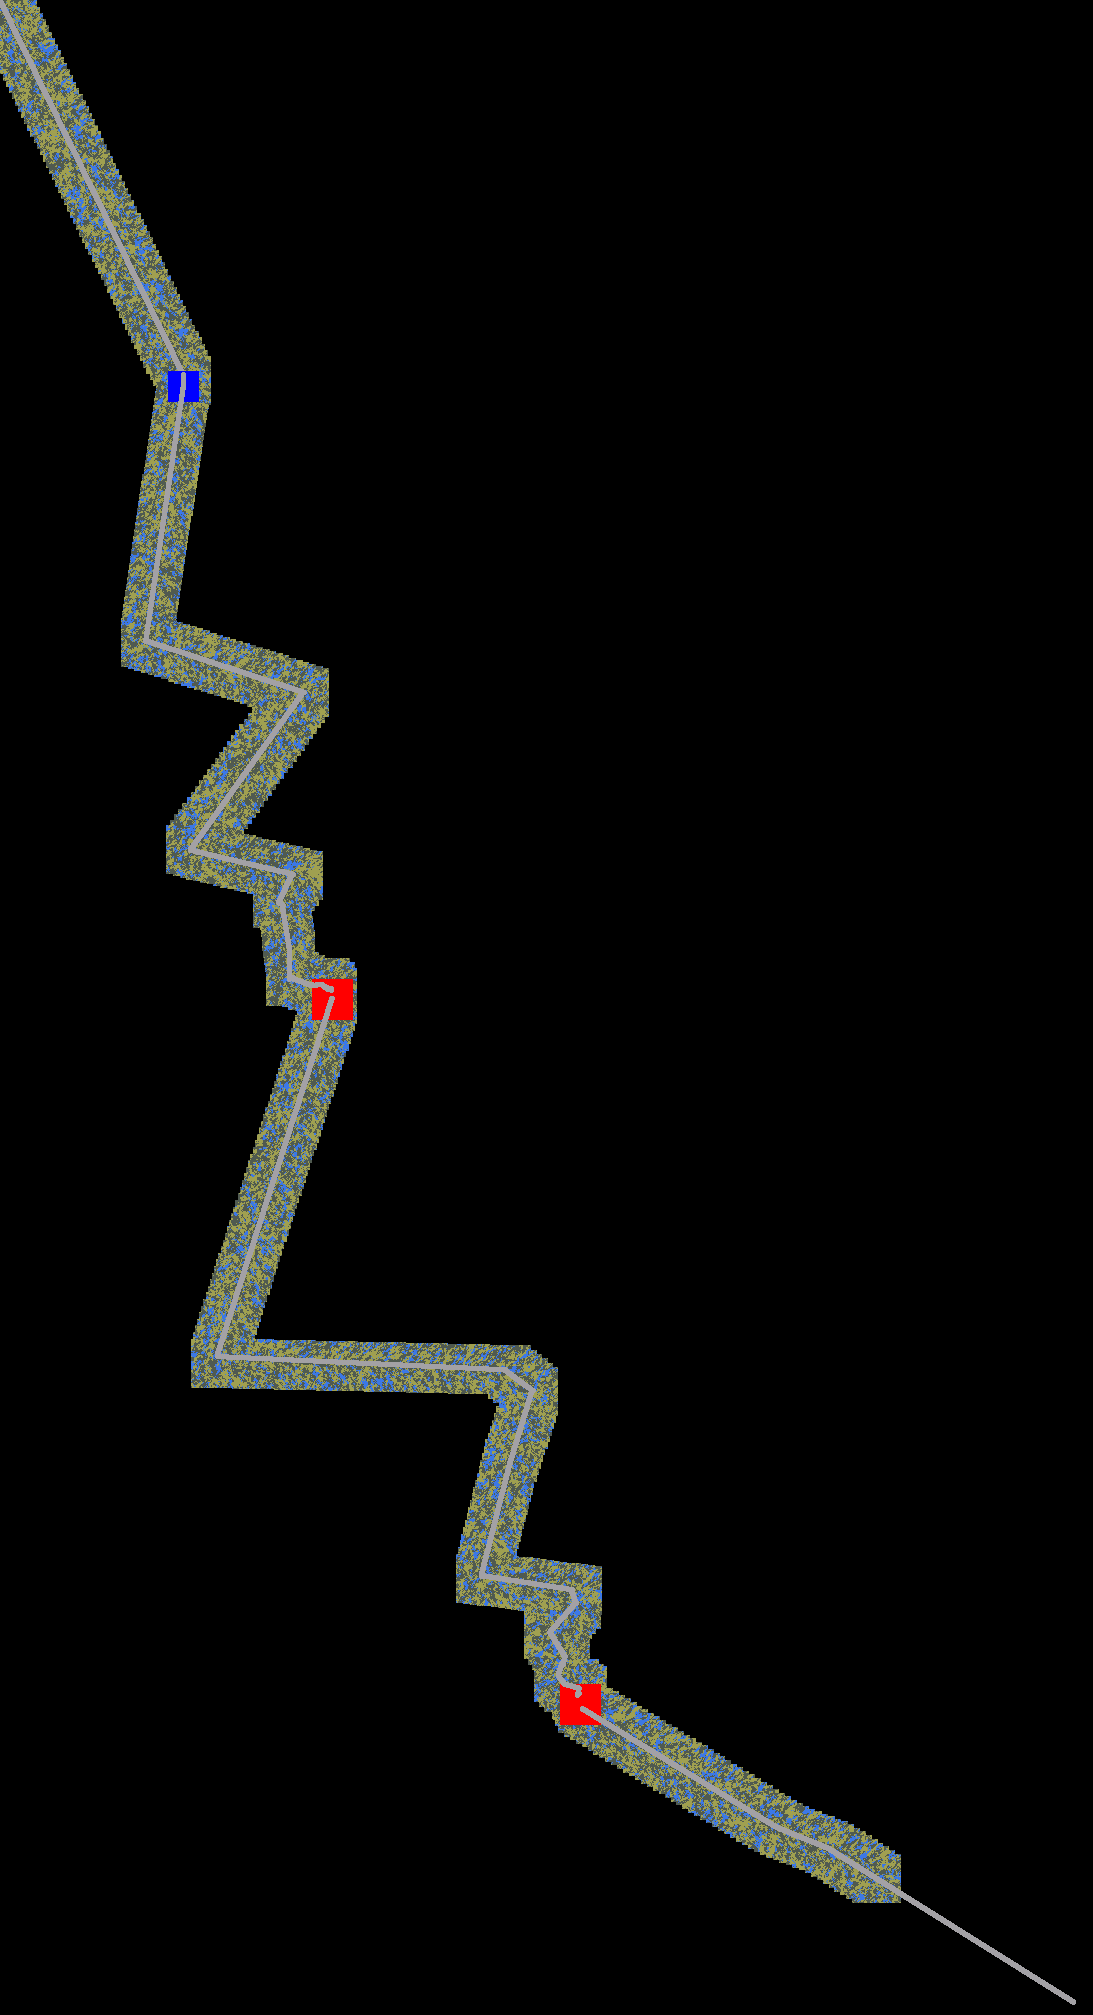
\includegraphics[height=0.7\paperheight]{map.png}
    \end{figure}
\end{frame}

\begin{frame}{Mutex}
    Utilisation raisonnable de mutex :
    \begin{itemize}
        \item Consomment beaucoup de ressources
        \item Vitesse, angle, niveau de batterie et position courante
        \item Compromis entre nombre de mutex et granularité
        \item Possibilité d’utiliser un seul
    \end{itemize}
    
    \bigskip
    
    \begin{itemize}
        \item[$\rightarrow$] Accès aux variables sécurisé
        \item[$\rightarrow$] Moins de conflits
    \end{itemize}
\end{frame}

\begin{frame}{Trace de données}
    \begin{itemize}
        \item Logs indispensables au débogage
        \item Fil d’exécution à 100ms
        \item Résultats
    \end{itemize}
\end{frame}

\begin{frame}{Trace de données}

\begin{columns}
    
    \begin{column}{0.5\paperwidth}
        \begin{figure}
            \centering
            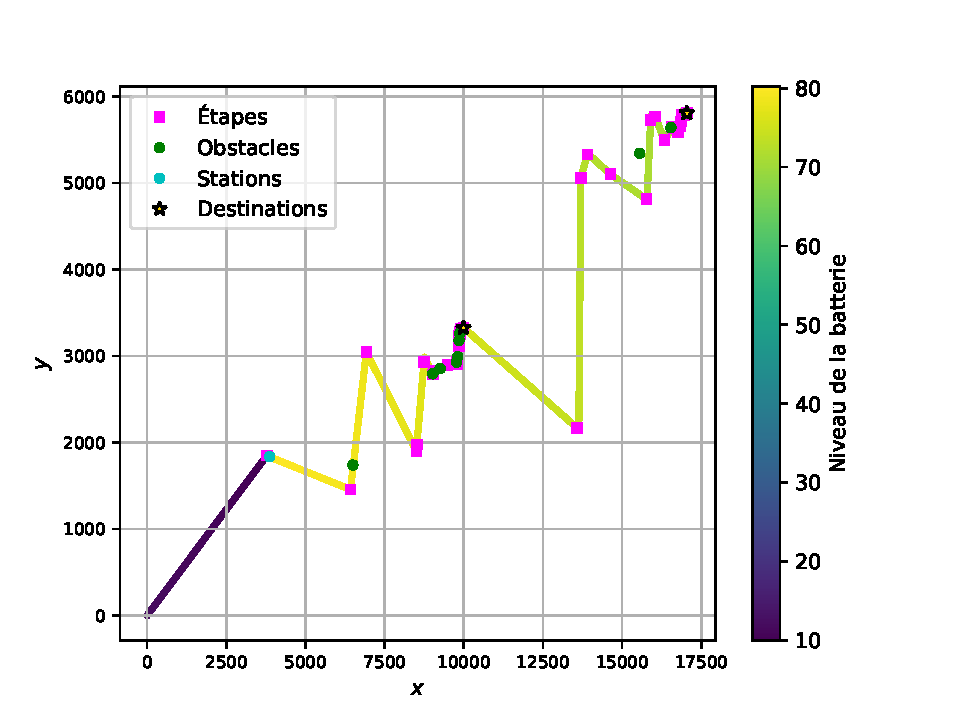
\includegraphics[width=0.55\paperwidth]{path.pdf}
            \caption{Chemin de la voiture et batterie}
        \end{figure}
    \end{column}
    
    \begin{column}{0.5\paperwidth}
       \begin{figure}
           \centering
           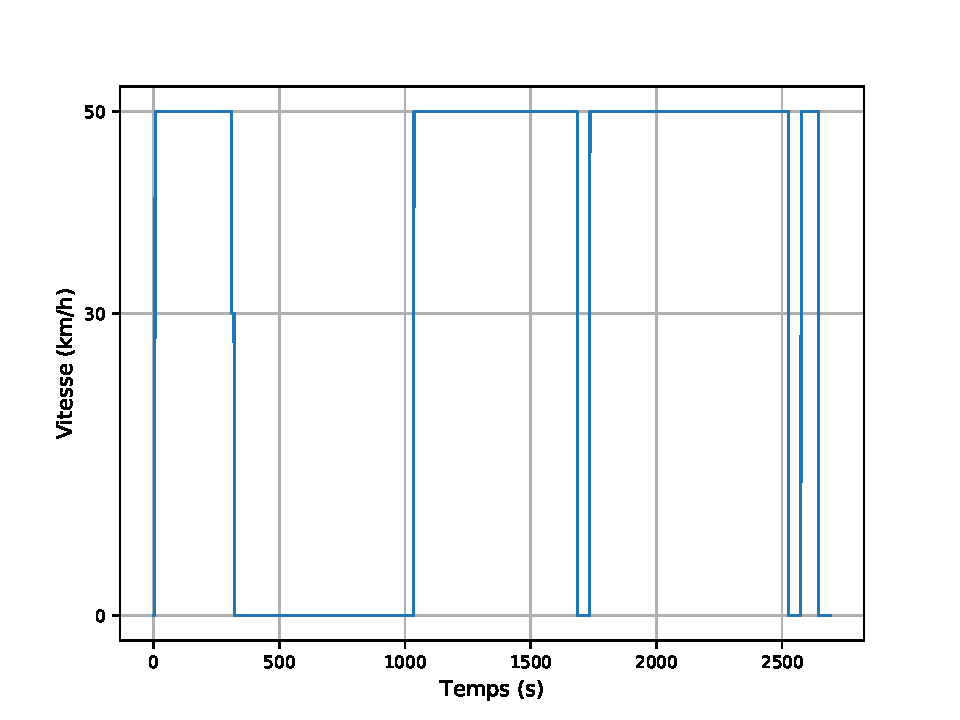
\includegraphics[width=0.55\paperwidth]{speed.pdf}
           \caption{Vitesse}
       \end{figure}
    \end{column}
    
\end{columns}

\end{frame}

\begin{frame}{Obstacles}

    \begin{columns}
    
    \begin{column}{0.45\paperwidth}
        \begin{itemize}
            \item Ajout d'états
            \item Plus réaliste
            \item Génération aléatoire
        \end{itemize}
    \end{column}
    
    \begin{column}{0.55\paperwidth}
    \begin{tikzpicture}[scale = 1]
    
    \tikzset{edge/.style = {->,> = latex'}}
    
    % vertices
	\node[rounded corners=3pt, draw=black, rectangle split, rectangle split parts = 2] (a)
		at  (-2,0) {\texttt{GOTO\_DEST} \nodepart{two} {\tiny vit. = 50km/h}};
	\node[rounded corners=3pt, draw=black, rectangle split, rectangle split parts = 2] (b)
		at  (2,0) {\texttt{PRE\_BATTLOW}\nodepart{two} {\tiny vit. = 30km/h}};
	\node[rounded corners=3pt, draw=black, rectangle split, rectangle split parts = 2] (c)
		at  (2,2) {\texttt{BATTLOW}\nodepart{two} {\tiny vit. = 30km/h}};
	\node[rounded corners=3pt, draw=black, rectangle split, rectangle split parts = 2] (d)
		at  (-2,2) {\texttt{CHARGING}\nodepart{two} {\tiny vit. = 0km/h}};
	\node[rounded corners=3pt, draw=black, rectangle split, rectangle split parts = 2] (e)
		at  (0,-2.7) {\texttt{PRE\_OBSTACLE}\nodepart{two} {\tiny vit. = 0km/h}};
	\node[rounded corners=3pt, draw=black, rectangle split, rectangle split parts = 2] (f)
		at  (0,-4.2) {\texttt{OBSTACLE}\nodepart{two} {\tiny vit. = 0km/h}};
    \node[circle, fill=black] (g) at (0,1) {};
    
    %edges
    \draw[edge] (g) to node [] {} (a);
    \draw[edge] (a) to node [above] {batt = 10} (b);
    \draw[edge] (b) to node [left] {} (c);
    \draw[edge] (c) to node [above] {closeTo(station)} (d);
    \draw[edge] (d) to node [left] {batt = 80} (a);
    \draw[edge] (a) to node [sloped, above] {\tiny closeTo(obstacle)} (e);
    \draw[edge] (b) to node [sloped, above] {\tiny closeTo(obstacle)} (e);
    \draw[edge] (e) to node [left] {} (f);
    \draw[edge] (f) to[bend left = 25] node [left] {!lowBat} (a);
    \draw[edge] (f) to[bend right = 25] node [right] {lowBat} (b);
    
    \end{tikzpicture}
    \end{column}
    
    \end{columns}

\end{frame}

\begin{frame}{Partitionnement CPU}

\begin{columns}
    
    \begin{column}{0.45\paperwidth}
        \begin{itemize}
            \item Mécanisme QNX
            \item Adaptatif
            \item Point critique des RTOS
            \item Deux partitions séparées:
            \begin{itemize}
                \item Tâches continues: 20\%
                \item Tâches discrètes: 60\%
            \end{itemize}
        \item Sécurité
        \end{itemize}
    \end{column}
    
    \begin{column}{0.55\paperwidth}
       \begin{figure}
           \centering
           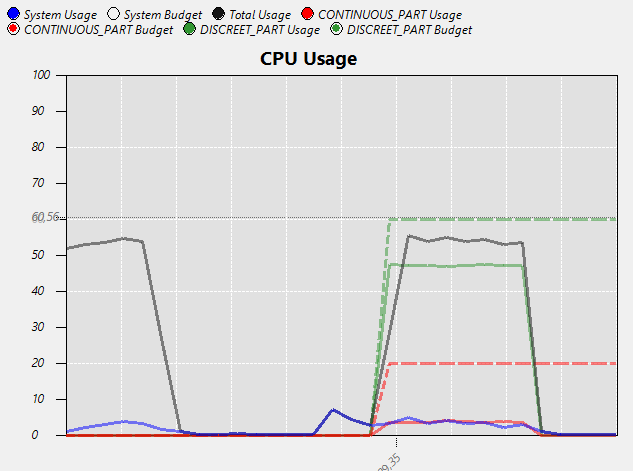
\includegraphics[width=0.5\paperwidth]{partitionnement.png}
           \caption{Partitionnement CPU}
       \end{figure}
    \end{column}
    
\end{columns}


    
    
\end{frame}

\section{Conclusion}

\begin{frame}{Conclusion}
    \begin{itemize}
        \item Comportement de la voiture autonome implémenté
        \item Enjeux du concept temps réel
        \item Solutions apportées aux problèmes rencontrés
        \item Système amélioré
        \begin{itemize}
            \item Fonctionnalités
            \item Performance
        \end{itemize}
        \item Résultats en simulation solides
        \item Pistes d’améliorations supplémentaires
         \begin{itemize}
            \item Affinité des threads
            \item Watchdogs
        \end{itemize}
    \end{itemize}
\end{frame}


\end{document}

% vim: set ts=4 sw=4 tw=90 noet :
